%%%%%%%%%%%%%%%%%%%%%%%%%%% asme2ej.tex %%%%%%%%%%%%%%%%%%%%%%%%%%%%%%%
% Template for producing ASME-format journal articles using LaTeX    %
% Written by   Harry H. Cheng, Professor and Director                %
%              Integration Engineering Laboratory                    %
%              Department of Mechanical and Aeronautical Engineering %
%              University of California                              %
%              Davis, CA 95616                                       %
%              Tel: (530) 752-5020 (office)                          %
%                   (530) 752-1028 (lab)                             %
%              Fax: (530) 752-4158                                   %
%              Email: hhcheng@ucdavis.edu                            %
%              WWW:   http://iel.ucdavis.edu/people/cheng.html       %
%              May 7, 1994                                           %
% Modified: February 16, 2001 by Harry H. Cheng                      %
% Modified: January  01, 2003 by Geoffrey R. Shiflett                %
% Use at your own risk, send complaints to /dev/null                 %
%%%%%%%%%%%%%%%%%%%%%%%%%%%%%%%%%%%%%%%%%%%%%%%%%%%%%%%%%%%%%%%%%%%%%%

%%% use twocolumn and 10pt options with the asme2ej format
\documentclass[twocolumn,10pt]{asme2ej}

\usepackage{graphicx} %% for loading jpg figures
\usepackage{url}
\usepackage{hyperref}
\usepackage{graphicx,animate}
\usepackage{float}

%% The class has several options
%  onecolumn/twocolumn - format for one or two columns per page
%  10pt/11pt/12pt - use 10, 11, or 12 point font
%  oneside/twoside - format for oneside/twosided printing
%  final/draft - format for final/draft copy
%  cleanfoot - take out copyright info in footer leave page number
%  cleanhead - take out the conference banner on the title page
%  titlepage/notitlepage - put in titlepage or leave out titlepage
%  
%% The default is oneside, onecolumn, 10pt, final


\title{Compressing Videos for video conferencing\\ - Name subject to change -}

%%% first author
\author{Antoine Buisson
    \affiliation{
	Graduate Student\\
	Department of Computer Science\\
	Seoul National University\\
	Télécom SudParis\\
    Email: abuisson@snu.ac.kr
    }	
}

%%% second author
%%% remove the following entry for single author papers
%%% add more entries for additional authors
\author{Mads Emil Marker Jungersen
    \affiliation{ 
    Undergraduate Student\\
	Department of Computer Science\\
	Seoul National University\\
	Aarhus University\\
    Email: madsjungersen@snu.ac.kr
    }
}

\author{Steve Suard
    \affiliation{ 
    Graduate Student\\
	Department of Computer Science\\
	Seoul National University\\
	Télécom SudParis\\
    Email: suard\_st@snu.ac.kr
    }
}

\author{Jonathan Åke Eun Woo Åkesson
    \affiliation{ 
    Graduate Student\\
	Department of ***********\\
	Seoul National University\\
	********************\\
    Email: j.akesson99@gmail.com
    }
}

\author{
    \affiliation{
    }
}








\begin{document}

\maketitle    

%%%%%%%%%%%%%%%%%%%%%%%%%%%%%%%%%%%%%%%%%%%%%%%%%%%%%%%%%%%%%%%%%%%%%%
\begin{abstract}
{\textit{
This paper proposes a low bandwidth talking-head video synthesis model (**MODEL NAME NOT YET CHOSEN**) for video conferencing. **MODEL NAME NOT YET CHOSEN** builds on the previous paper "One-Shot Free-View Neural Talking-Head Synthesis for Video Conferencing" (face-vid2vid). We decided to work on the Source Image. The main idea is to send through the internet a low resolution resized version of the source image and upscale it at the other end with a super resolution model from the paper "Enhanced Super-Resolution Generative Adversarial Networks" (ESRGAN). The goal is to either to reduce the amount of bandwidth needed, or be able to send more Source Images without impacting the bandwidth.
} }
\end{abstract}

%%%%%%%%%%%%%%%%%%%%%%%%%%%%%%%%%%%%%%%%%%%%%%%%%%%%%%%%%%%%%%%%%%%%%%
%\begin{nomenclature}
%\entry{A}{You may include nomenclature here.}
%\entry{$\alpha$}{There are two arguments for each entry of the nomemclature environment, the symbol and the definition.}
%\end{nomenclature}
%
%The primary text heading is  boldface and flushed left with the left margin.  The spacing between the  text and the heading is two line spaces.

%%%%%%%%%%%%%%%%%%%%%%%%%%%%%%%%%%%%%%%%%%%%%%%%%%%%%%%%%%%%%%%%%%%%%%
\section{Introduction}

Due to the COVID-19 Pandemic and the rise of new technology, videoconference is becoming a standard in every industry and in education. As Humans, we have a need for facial communication, this explain why it is now a standard to share your face through your webcam during such videoconferences. But this lead to two major problems. First of all, video data is the data type that use the internet bandwidth the most. Secondly, some workers and student may not have the best internet connection and will sometime experience connection drops when many people are sharing their webcams.
That is why we should find a way to optimize the amount of data needed to share your face for videoconferences.

One of the proposed methods is the Talking-Head Video Synthesis. The idea is to take a high quality source image. Only use the driving video from the webcam to extract a number of facial feature. And finnaly reconstruct the video by morphing the features on the source image. This work extremely great to reduce the bandwidth. But reconstructing a whole video from a single image can lead to erroned results when the driving position from the video is becoming too different from the original Source Image position.

Another proposed method is the use of Super resolution models. The idea would be to only send a low resolution driving video through the internet, and upscale it back to its original resolution before being displayed. The main issue with this is that Super resolution models are usually pretty slow for good looking results and that it is sometimes hard to keep a temporal stability between each frame, which lead to a lot of flickering.

Having look at these two solutions, our idea is to use the best of both worlds by adding a super resolution block in the Talking-Head Video Synthesis Model. This could lead to more Sources Images being sent and thus, bring a solution to the previous erroneous results.

%%%%%%%%%%%%%%%%%%%%%%%%%%%%%%%%%%%%%%%%%%%%%%%%%%%%%%%%%%%%%%%%%%%%%%
\section{Literature Survey}

%%%%%%%%%%%%%%%%%%%%%%%%%%%%%%%%%%%%%%%%%%%%%%%%%%%%%%%%%%%%%%%%%%%%%%
\subsection{One-Shot Free-View Neural Talking-Head Synthesis for Video Conferencing}

This is the main building block for our solution. This paper was written by Ting-Chun Wang, Arun Mallya and Ming-Yu Liu from NVIDIA Corporation. Their methods allowed similar video results with H264 but for only one tenth of the bit rate. This paper is also able to re-render novel-view, meaning it can change the head position and rotation if needed [ref Fig~\ref{fig_face_vid2vid.png}]. Finally, all those functions allow the model to do deepfake by simply choosing 2 different persons for the Source Image and Driving Image.

Here is the link to their paper : \href{https://nvlabs.github.io/face-vid2vid/}{nvlabs.github.io/face-vid2vid}

\begin{figure} 
\centerline{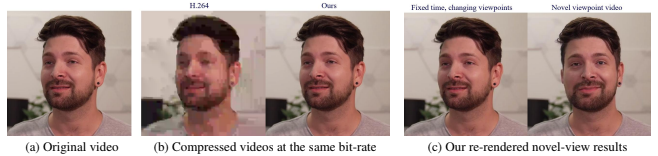
\includegraphics[width=3.34in]{figure/face_vid2vid.png}}
\caption{Face\_vid2vid article preview}
\label{fig_face_vid2vid.png}
\end{figure}


%%%%%%%%%%%%%%%%%%%%%%%%%%%%%%%%%%%%%%%%%%%%%%%%%%%%%%%%%%%%%%%%%%%%%%
\subsection{Enhanced Super-Resolution Generative Adversarial Networks}

This is the block that we wish to add to the face\_vid2vid network. This paper was written by Xintao Wang, Ke Yu, Shixiang Wu
,Jinjin Gu, Yihao Liu, Chao Dong, Chen Change Loy, Yu Qiao and Xiaoou Tang. Their solution build on the previous SRGAN paper that was capable of generating realistic textures during single image super-resolution.

Here is the link to their paper : \href{https://arxiv.org/pdf/1809.00219.pdf}{1809.00219.pdf}

%%%%%%%%%%%%%%%%%%%%%%%%%%%%%%%%%%%%%%%%%%%%%%%%%%%%%%%%%%%%%%%%%%%%%%
\section{Data Pipeline}

We need images or videos of talking human faces. This is a common type of data to be found, and thus many datasets already exist.
We choose the VoxCeleb2 Dataset with 6000 speakers and around 150000 videos. This is one of the most used Dataset which might help us for the baselines.\\
VoxCeleb2 : \href{https://www.robots.ox.ac.uk/~vgg/data/voxceleb/vox2.html}{robots.ox.ac.uk/~vgg/data/voxceleb/vox2.html}


In the NVIDIA Research paper, the researchers are talking about a new dataset they created called TalkingHead-
1KH with 180000 new videos or higher quality and larger resolution than VoxCeleb2. This is still a private dataset from NVIDIA but we might be able to get our hand on it.

Still, we do not have enough computational power to handle such datasets, meaning we decided to only use a small part of the whole dataset. Moreover, video used for video-conferencing isn't usually in ultra high quality so we can restrain ourselves from using 4K videos.

Finally, the researchers of face\_vid2vid paper trained their model on a NVIDIA DGX1 with 8 32GB V100 GPUs and using more than 250K videos with high bit rates. Not having the computational power as well as the time, we decided to only do fine tuning (if necessary) on the already existing model.

%%%%%%%%%%%%%%%%%%%%%%%%%%%%%%%%%%%%%%%%%%%%%%%%%%%%%%%%%%%%%%%%%%%%%%
\section{Our Solution\protect\footnotemark}
\footnotetext{Still need all the training and merging of the two solution}

At the end of our research project, we aim to have both the Talking-Head Video Synthesis Model and Single Image Super Resolution Model as one. To create an upgraded version of face\_vid2vid.
For now, we only have these two networks on their one, but we will discuss where we are at in the next 2 subsections.

\subsection{Talking-Head Video Synthesis Model}
An unofficial implementation of the model proposed in the face-vid2vid is available at  \href{https://github.com/zhanglonghao1992/One-Shot_Free-View_Neural_Talking_Head_Synthesis?ref=pythonrepo.com}{Github}, where pretrained weights from the VoxCeleb-v1 dataset is available for download as well. We implemented the model, loaded the pretrained weights, and were able to run inference with a self-chosen driving video and source image. The result of this inference can be seen in figure \ref{AnimationInf} (open in Adobe Reader to show animation). The pretrained model used has not been well tuned (according to the author), and a natural next step would be to fine-tune the model on our dataset. Running inference on the current model takes approximately 3-6 minutes, which is a challenge since the goal of the model is to be able to run in something near real-time. However we tried different driving videos and source images and in every case the output showed promising results. A future challenge therefore is to reduce the inference time, as well as to find good metrics to measure the quality of the out from the model. Some metrics are proposed in the face-vid2vid and these would be implemented as metrics to compare our final model with below-mentioned benchmarks.    



\begin{figure}[H] 
\centerline{\animategraphics[loop,autoplay,scale=0.20]{10}{"gif1/frame_"}{0}{25}}
\caption{Animated output from running inference on face\_vid2vid implementation (open in Adobe Reader)}
\label{AnimationInf}
\end{figure}

\subsection{Single Image Super Resolution Model}

Code link : \href{https://github.com/xinntao/ESRGAN}{https://github.com/xinntao/ESRGAN}

This is the original code and model from ESRGAN article. The models given were trained using the OST dataset (outdoor scenes) and DF2K dataset (various photos from Flickr). It also implement the REAL-ESRGAN algorithm which aim to remove artefact compression from real-world images. We will try to use them both to see which one give better results for faces. We will also try to fine-tune it using the vox-celeb dataset, to see if we could achieve better looking results for video conferencing images.

%%%%%%%%%%%%%%%%%%%%%%%%%%%%%%%%%%%%%%%%%%%%%%%%%%%%%%%%%%%%%%%%%%%%%%
\section{Implemented Baselines}

\subsection{Talking-Head Video Synthesis Model}

\subsubsection{First Order Motion Model for Image Animation [FOMM]}

Paper link : \href{https://proceedings.neurips.cc/paper/2019/file/31c0b36aef265d9221af80872ceb62f9-Paper.pdf}{https://proceedings.neurips.cc/paper/...}

Code link : \href{https://github.com/AliaksandrSiarohin/first-order-model}{https://github.com/AliaksandrSiarohin/...}

\subsubsection{Fast Bi-layer Neural Synthesis of One-Shot
Realistic Head Avatars}

Paper link : \href{https://arxiv.org/pdf/2008.10174.pdf}{https://arxiv.org/pdf/2008.10174.pdf}

Code link : \href{https://github.com/saic-violet/bilayer-model}{https://github.com/saic-violet/bilayer-model}

\subsection{Single Image Super Resolution Model}
A model for single-image super resolution has been implemented using Tensorflow Hub's implementation of ESRGAN. The model is trained to upscale 128x128 pixel images by 4 times, on the div2k dataset. This model was experimented with on the Tensorflow dataset ''aflw2k3d'', which contains images and data on faces and different facial landmarks (only the images was used). The images of size 450x450 pixels was firstly downsampled to 128x128 pixels and the upsampled four times to 512x512 pixels using the model. The results from this can be seen in figure \ref{ESRGAN_comp}. When upscaling the images using this model the inference time is around 2.5 s per image (using virtual GPU in google collab). Other order of magnifications that has been tested are 1/6 and 1/8 of the original image scale. The output images was however clearly distinguishable from the original images in these cases. This might be due to the size and content of the images in the training data. It is possible to retrain the model, but it will also require implementation of a new discriminator. An implementation of Super Resolution GAN (SRGAN) has also been attempted to implement, but not yet with comparable result to the ESRGAN. While the current ESRGAN model gives very good result when upscaling images under certain conditions, it might need some tweaks to enhance the talking head synthesis model. Things that might have to be improved is the possible input scales and possibility to upscale by bigger magnitudes than four.

\begin{figure}[H]
    \centering
    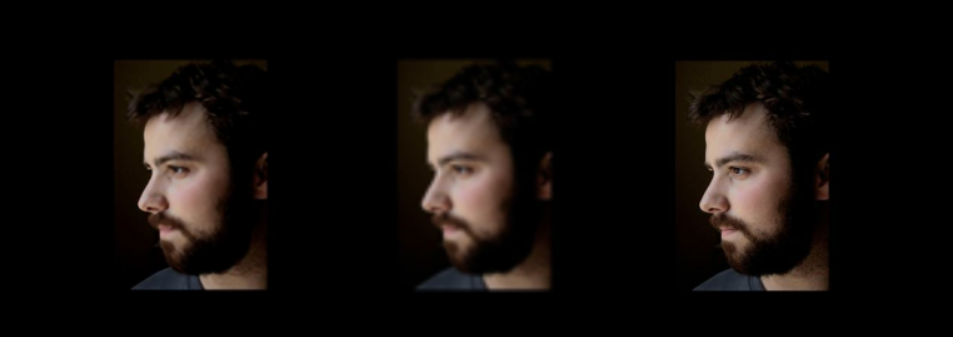
\includegraphics[width=\textwidth/2]{ESRGAN_comparison.png}
    \caption{Left: Upscaled image using Tensorflow Hub's ESRGAN implementation\\
    Middle: Image compressed to one fourth of the size and then resized to 512x512 pixels\\
    Right: Original image}
    \label{ESRGAN_comp}
\end{figure}

\subsubsection{Enhanced Deep Residual Networks for Single Image Super-Resolution [EDSR]}

Paper link : \href{https://arxiv.org/pdf/1707.02921.pdf}{https://arxiv.org/pdf/1707.02921.pdf}

Code link : \href{https://github.com/Saafke/EDSR_Tensorflow}{https://github.com/Saafke/EDSR_Tensorflow}


\end{document}
